\documentclass[border=3pt]{standalone}
% Preâmbulo compartilhado pelos diagramas TikZ da aula 4 de Navegação (Representação de Mapas)
\usepackage[T1]{fontenc}
\usepackage[utf8]{inputenc}
\usepackage{lmodern}
\usepackage{amsmath}
\usepackage{xcolor}
\usepackage{tikz}
\usetikzlibrary{arrows.meta,angles,quotes,decorations.pathmorphing,decorations.pathreplacing,calc,
                positioning,shapes.geometric,shapes.misc,backgrounds,fit,
                math}

% Paleta (mesma dos SVGs originais)
\definecolor{dblue}{HTML}{2A5B8C}
\definecolor{dorange}{HTML}{B3541E}
\definecolor{dgreen}{HTML}{4A7C59}
\definecolor{dred}{HTML}{9C4B4B}
\definecolor{dcream}{HTML}{F4F1EA}
\definecolor{dshade}{HTML}{DDD7C9}

% Função gaussiana (não normalizada por padrão de escala visual)
\pgfmathdeclarefunction{gauss}{3}{%
  \pgfmathparse{1/(#3*sqrt(2*pi))*exp(-((#1-#2)^2)/(2*#3^2))}%
}

% Estilos comuns (prefixo d... para não colidir com chaves internas do pgf)
\tikzset{
  >={Stealth[length=2mm]},
  dguide/.style={gray!55, dashed, line width=0.4pt},
  daxis/.style={gray!60, line width=0.7pt, ->},
  dbody/.style={fill=black!3, draw=black!80, line width=1pt},
  dacc/.style={draw=dblue, line width=1pt},
  dlbl/.style={black!55, font=\small},
  dsub/.style={black!45, font=\footnotesize},
  dstate/.style={circle, draw=black!80, fill=dcream, line width=1pt,
                 minimum size=17mm, font=\large, inner sep=1pt},
  dobs/.style={circle, draw=black!80, fill=dshade, line width=1pt,
               minimum size=14mm, font=\large, inner sep=1pt},
  dbox/.style={rounded corners=2pt, draw=black!80, fill=dcream, line width=1pt,
               align=center, inner sep=6pt},
  dop/.style={circle, draw=black!80, fill=white, line width=1pt,
              minimum size=6mm, inner sep=0pt, font=\small},
  dtrans/.style={->, dblue, line width=1pt},
  dmeas/.style={->, dorange, line width=1pt},
  dcurve/.style={line width=1pt, dblue},
  dcurveb/.style={line width=1.4pt, dorange},
}

\begin{document}
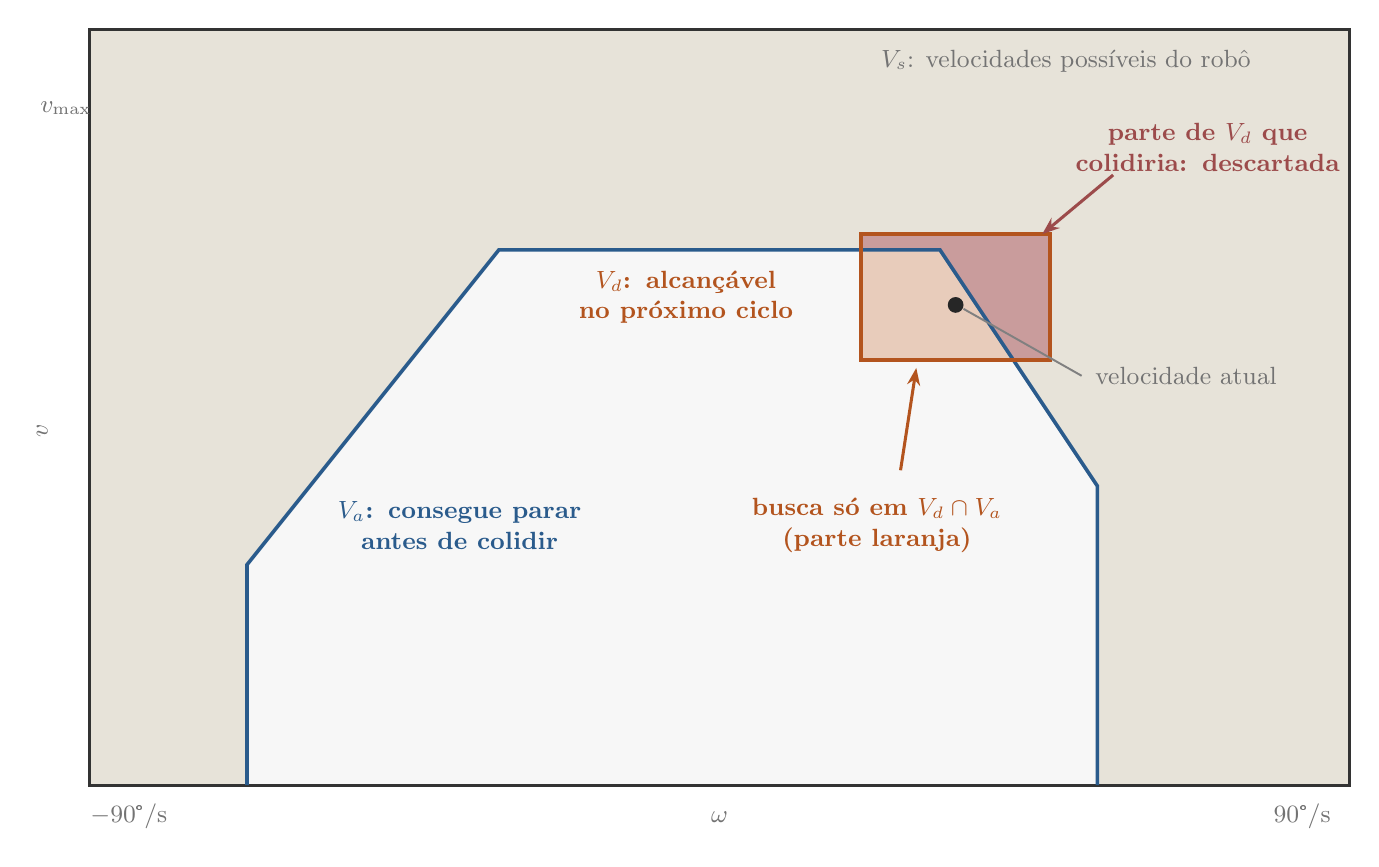
\begin{tikzpicture}[x=1cm,y=1cm]

  % V_s: todo o espaço; fora de V_a fica sombreado (colidiria)
  \fill[dshade!70!white] (0,0) rectangle (16,9.6);
  \fill[black!3] (2.0,0) -- (2.0,2.8) -- (5.2,6.8) -- (10.8,6.8) -- (12.8,3.8) -- (12.8,0) -- cycle;
  \draw[black!80, line width=1.2pt] (0,0) rectangle (16,9.6);
  \node[dlbl, font=\small] at (12.4,9.2) {$V_s$: velocidades possíveis do robô};

  % janela dinâmica V_d (retângulo em torno da velocidade atual) cruzando a fronteira de V_a
  \def\xa{9.8}\def\xb{12.2}\def\ya{5.4}\def\yb{7.0}
  % parte de V_d dentro de V_a (interseção, onde se busca)
  \begin{scope}
    \clip (2.0,0) -- (2.0,2.8) -- (5.2,6.8) -- (10.8,6.8) -- (12.8,3.8) -- (12.8,0) -- cycle;
    \fill[dorange!30!white] (\xa,\ya) rectangle (\xb,\yb);
  \end{scope}
  % parte de V_d fora de V_a (colidiria)
  \begin{scope}
    \clip (\xa,\ya) rectangle (\xb,\yb);
    \fill[dred!55!white] (0,0) rectangle (16,9.6);
    \fill[dorange!30!white] (2.0,0) -- (2.0,2.8) -- (5.2,6.8) -- (10.8,6.8) -- (12.8,3.8) -- (12.8,0) -- cycle;
  \end{scope}
  \draw[dblue, line width=1.3pt] (2.0,0) -- (2.0,2.8) -- (5.2,6.8) -- (10.8,6.8) -- (12.8,3.8) -- (12.8,0);
  \draw[dorange, line width=1.5pt] (\xa,\ya) rectangle (\xb,\yb);

  % velocidade atual
  \fill[black!85] (11.0,6.1) circle (0.1);
  \draw[black!50, line width=0.7pt] (11.1,6.05) -- (12.6,5.2);
  \node[dlbl, font=\small, anchor=west] at (12.65,5.2) {velocidade atual};

  % rótulos
  \node[dblue, font=\small\bfseries, align=center, text width=3.2cm] at (4.7,3.3) {$V_a$: consegue parar antes de colidir};
  \node[dorange, font=\small\bfseries, align=center, anchor=east, text width=3.6cm] at (9.5,6.2) {$V_d$: alcançável no próximo ciclo};
  \node[dorange, font=\small\bfseries, align=center, text width=3.6cm] at (10.0,3.3) {busca só em $V_d \cap V_a$ (parte laranja)};
  \draw[dorange, line width=1.1pt, -{Stealth[length=2.2mm]}] (10.3,4.0) -- (10.5,5.3);
  \node[dred, font=\small\bfseries, align=center, text width=3.4cm] at (14.2,8.1) {parte de $V_d$ que colidiria: descartada};
  \draw[dred, line width=1.1pt, -{Stealth[length=2.2mm]}] (13.0,7.75) -- (12.1,7.0);

  \node[dlbl, font=\small] at (0.5,-0.4) {$-90${\textdegree}/s};
  \node[dlbl, font=\small] at (8,-0.4) {$\omega$};
  \node[dlbl, font=\small] at (15.4,-0.4) {$90${\textdegree}/s};
  \node[dlbl, font=\small, rotate=90] at (-0.6,4.5) {$v$};
  \node[dlbl, font=\small] at (-0.3,8.6) {$v_{\max}$};

\end{tikzpicture}
\end{document}
